\documentclass[a4paper,12pt,twoside]{report}
\usepackage[left=2cm,right=2cm,top=2cm,bottom=3cm]{geometry}
\usepackage[final]{pdfpages}
\usepackage{cite}
\usepackage{subfig}
\usepackage{url}
\usepackage{wasysym}
\usepackage{amssymb}
\usepackage{emptypage}

\usepackage{graphicx}
\usepackage{verbatim}
\usepackage{latexsym}
\usepackage{mathchars}
\usepackage{setspace}

\setlength{\parskip}{\medskipamount}  % a little space before a \par
\setlength{\parindent}{0pt}	      % don't indent first lines of paragraphs
%UHEAD.STY  If this is included after \documentstyle{report}, it adds
% an underlined heading style to the LaTeX report style.
% \pagestyle{uheadings} will put underlined headings at the top
% of each page. The right page headings are the Chapter titles and
% the left page titles are supplied by \def\lefthead{text}.

% Ted Shapin, Dec. 17, 1986

\makeatletter
\def\chapapp2{Chapter}

\def\appendix{\par
 \setcounter{chapter}{0}
 \setcounter{section}{0}
 \def\chapapp2{Appendix}
 \def\@chapapp{Appendix}
 \def\thechapter{\Alph{chapter}}}

\def\ps@uheadings{\let\@mkboth\markboth
% modifications
\def\@oddhead{\protect\underline{\protect\makebox[\textwidth][l]
		{\sl\rightmark\hfill\rm\thepage}}}
\def\@oddfoot{}
\def\@evenfoot{}
\def\@evenhead{\protect\underline{\protect\makebox[\textwidth][l]
		{\rm\thepage\hfill\sl\leftmark}}}
% end of modifications
\def\chaptermark##1{\markboth {\ifnum \c@secnumdepth >\m@ne
 \chapapp2\ \thechapter. \ \fi ##1}{}}%
\def\sectionmark##1{\markright {\ifnum \c@secnumdepth >\z@
   \thesection. \ \fi ##1}}}
\makeatother
%%From: marcel@cs.caltech.edu (Marcel van der Goot)
%%Newsgroups: comp.text.tex
%%Subject: illegal modification of boxit.sty
%%Date: 28 Feb 92 01:10:02 GMT
%%Organization: California Institute of Technology (CS dept)
%%Nntp-Posting-Host: andromeda.cs.caltech.edu
%%
%%
%%Quite some time ago I posted a file boxit.sty; maybe it made it
%%to some archives, although I don't recall submitting it. It defines
%%	\begin{boxit}
%%	...
%%	\end{boxit}
%%to draw a box around `...', where the `...' can contain other
%%environments (e.g., a verbatim environment). Unfortunately, it had
%%a problem: it did not work if you used it in paragraph mode, i.e., it
%%only worked if there was an empty line in front of \begin{boxit}.
%%Luckily, that is easily corrected.
%%
%%HOWEVER, apparently someone noticed the problem, tried to correct it,
%%and then distributed this modified version. That would be fine with me,
%%except that:
%%1. There was no note in the file about this modification, it only has my
%%   name in it.
%%2. The modification is wrong: now it only works if there is *no* empty
%%   line in front of \begin{boxit}. In my opinion this bug is worse than
%%   the original one.
%%
%%In particular, the author of this modification tried to force an empty
%%line by inserting a `\\' in the definition of \Beginboxit. If you have
%%a version of boxit.sty with a `\\', please delete it. If you have my
%%old version of boxit.sty, please also delete it. Below is an improved
%%version.
%%
%%Thanks to Joe Armstrong for drawing my attention to the bug and to the
%%illegal version.
%%
%%                                          Marcel van der Goot
%% .---------------------------------------------------------------
%% | Blauw de viooltjes,                    marcel@cs.caltech.edu
%% |    Rood zijn de rozen;
%% | Een rijm kan gezet
%% |    Met plaksel en dozen.
%% |


% boxit.sty
% version: 27 Feb 1992
%
% Defines a boxit environment, which draws lines around its contents.
% Usage:
%   \begin{boxit}
%	... (text you want to be boxed, can contain other environments)
%   \end{boxit}
%
% The width of the box is the width of the contents.
% The boxit* environment behaves the same, except that the box will be
% at least as wide as a normal paragraph.
%
% The reason for writing it this way (rather than with the \boxit#1 macro
% from the TeXbook), is that now you can box verbatim text, as in
%   \begin{boxit}
%   \begin{verbatim}
%   this better come out in boxed verbatim mode ...
%   \end{verbatim}
%   \end{boxit}
%
%						Marcel van der Goot
%						marcel@cs.caltech.edu
%

\def\Beginboxit
   {\par
    \vbox\bgroup
	   \hrule
	   \hbox\bgroup
		  \vrule \kern1.2pt %
		  \vbox\bgroup\kern1.2pt
   }

\def\Endboxit{%
			      \kern1.2pt
		       \egroup
		  \kern1.2pt\vrule
		\egroup
	   \hrule
	 \egroup
   }	

\newenvironment{boxit}{\Beginboxit}{\Endboxit}
\newenvironment{boxit*}{\Beginboxit\hbox to\hsize{}}{\Endboxit}
\pagestyle{empty}

\setlength{\parskip}{2ex plus 0.5ex minus 0.2ex}
\setlength{\parindent}{0pt}

\makeatletter  %to avoid error messages generated by "\@". Makes Latex treat "@" like a letter

\linespread{1.5}
\def\submitdate#1{\gdef\@submitdate{#1}}

\def\supervisor#1{\gdef\@supervisor{#1}}

\def\maketitle{
  \begin{titlepage}{
    %\linespread{1.5}

    \rm
    \vskip 3in
    \Large \bf \@title \par
  }
  \par
    Thesis for the degree of
  \linebreak
    “Doctor of Philosophy”
  \vskip 0.3in
  \par
  By
  \linebreak
  \vskip 0.3in
  {\Large \@author}
  \vskip 4in
  \par
  Submitted to the Senate of the Hebrew University of Jerusalem
  \linebreak
  \@submitdate
  \vfil
  \end{titlepage}
}

\def\titlepage{
  \newpage
  \centering
  \linespread{1}
  \normalsize
  \vbox to \vsize\bgroup\vbox to 9in\bgroup
}
\def\endtitlepage{
  \par
  \kern 0pt
  \egroup
  \vss
  \egroup
  \cleardoublepage
}


\def\supervised{
  \begin{center}{
    \small This work was carried out under the supervision of:
      \linebreak
      \large
      \@supervisor
  }
  \end{center}
  %\def\baselinestretch{1.5}
  \linespread{1.5}
  \cleardoublepage
  \normalsize
}
\def\endsupervised{
  \par
  \cleardoublepage
}

\def\abstract{
  \begin{center}{
    \large\bf Abstract}
  \end{center}
  \small
  %\def\baselinestretch{1.5}
  \linespread{1.5}
  \normalsize
}
\def\endabstract{
  \par
}

\newenvironment{acknowledgements}{
  \begin{center}{
    \large \bf Acknowledgements}
  \end{center}
  \small
  \linespread{1.5}
  \normalsize
}
\def\endacknowledgements{
  \par
}

\newenvironment{contributions}{
  \begin{center}{
    \large \bf Letter of Contributions}
  \end{center}
  \small
  \linespread{1.5}
  \normalsize
}
\def\endcontributions{
  \par
}

\def\preface{
    \pagenumbering{roman}
    \pagestyle{plain}
    \doublespacing
}


\def\body{
    \cleardoublepage    
    \pagestyle{uheadings}
    \tableofcontents
    \pagestyle{plain}
    \cleardoublepage
%    \pagestyle{uheadings}
%    \listoftables
%    \pagestyle{plain}
%    \cleardoublepage
%    \pagestyle{uheadings}
%    \listoffigures
    \pagestyle{plain}
    \cleardoublepage
    \pagestyle{uheadings}
    \pagenumbering{arabic}
    \doublespacing
}

\def\addpdfchapter[#1]#2#3{
    \newpage
    \chapter{#1}\label{#3}
    \par #2
    \pagestyle{plain}
    \cleardoublepage
    \includepdf[pages=-]{#3}
}

\makeatother  %to avoid error messages generated by "\@". Makes Latex treat "@" like a letter

\newcommand{\ipc}{{\sf ipc}}

\newcommand{\Prob}{\bbbp}
\newcommand{\Real}{\bbbr}
\newcommand{\real}{\Real}
\newcommand{\Int}{\bbbz}
\newcommand{\Nat}{\bbbn}

\newcommand{\NN}{{\sf I\kern-0.14emN}}   % Natural numbers
\newcommand{\ZZ}{{\sf Z\kern-0.45emZ}}   % Integers
\newcommand{\QQQ}{{\sf C\kern-0.48emQ}}   % Rational numbers
\newcommand{\RR}{{\sf I\kern-0.14emR}}   % Real numbers
\newcommand{\KK}{{\cal K}}
\newcommand{\OO}{{\cal O}}
\newcommand{\AAA}{{\bf A}}
\newcommand{\HH}{{\bf H}}
\newcommand{\II}{{\bf I}}
\newcommand{\LL}{{\bf L}}
\newcommand{\PP}{{\bf P}}
\newcommand{\PPprime}{{\bf P'}}
\newcommand{\QQ}{{\bf Q}}
\newcommand{\UU}{{\bf U}}
\newcommand{\UUprime}{{\bf U'}}
\newcommand{\zzero}{{\bf 0}}
\newcommand{\ppi}{\mbox{\boldmath $\pi$}}
\newcommand{\aalph}{\mbox{\boldmath $\alpha$}}
\newcommand{\bb}{{\bf b}}
\newcommand{\ee}{{\bf e}}
\newcommand{\mmu}{\mbox{\boldmath $\mu$}}
\newcommand{\vv}{{\bf v}}
\newcommand{\xx}{{\bf x}}
\newcommand{\yy}{{\bf y}}
\newcommand{\zz}{{\bf z}}
\newcommand{\oomeg}{\mbox{\boldmath $\omega$}}
\newcommand{\res}{{\bf res}}
\newcommand{\cchi}{{\mbox{\raisebox{.4ex}{$\chi$}}}}
%\newcommand{\cchi}{{\cal X}}
%\newcommand{\cchi}{\mbox{\Large $\chi$}}

% Logical operators and symbols
\newcommand{\imply}{\Rightarrow}
\newcommand{\bimply}{\Leftrightarrow}
\newcommand{\union}{\cup}
\newcommand{\intersect}{\cap}
\newcommand{\boolor}{\vee}
\newcommand{\booland}{\wedge}
\newcommand{\boolimply}{\imply}
\newcommand{\boolbimply}{\bimply}
\newcommand{\boolnot}{\neg}
\newcommand{\boolsat}{\!\models}
\newcommand{\boolnsat}{\!\not\models}


\newcommand{\op}[1]{\mathrm{#1}}
\newcommand{\s}[1]{\ensuremath{\mathcal #1}}

% Properly styled differentiation and integration operators
\newcommand{\diff}[1]{\mathrm{\frac{d}{d\mathit{#1}}}}
\newcommand{\diffII}[1]{\mathrm{\frac{d^2}{d\mathit{#1}^2}}}
\newcommand{\intg}[4]{\int_{#3}^{#4} #1 \, \mathrm{d}#2}
\newcommand{\intgd}[4]{\int\!\!\!\!\int_{#4} #1 \, \mathrm{d}#2 \, \mathrm{d}#3}

% Large () brackets on different lines of an eqnarray environment
\newcommand{\Leftbrace}[1]{\left(\raisebox{0mm}[#1][#1]{}\right.}
\newcommand{\Rightbrace}[1]{\left.\raisebox{0mm}[#1][#1]{}\right)}

% Funky symobols for footnotes
\newcommand{\symbolfootnote}{\renewcommand{\thefootnote}{\fnsymbol{footnote}}}
% now add \symbolfootnote to the beginning of the document...

\newcommand{\normallinespacing}{\renewcommand{\baselinestretch}{1.5} \normalsize}
\newcommand{\mediumlinespacing}{\renewcommand{\baselinestretch}{1.2} \normalsize}
\newcommand{\narrowlinespacing}{\renewcommand{\baselinestretch}{1.0} \normalsize}
\newcommand{\bump}{\noalign{\vspace*{\doublerulesep}}}
\newcommand{\cell}{\multicolumn{1}{}{}}
\newcommand{\spann}{\mbox{span}}
\newcommand{\diagg}{\mbox{diag}}
\newcommand{\modd}{\mbox{mod}}
\newcommand{\minn}{\mbox{min}}
\newcommand{\andd}{\mbox{and}}
\newcommand{\forr}{\mbox{for}}
\newcommand{\EE}{\mbox{E}}

\newcommand{\deff}{\stackrel{\mathrm{def}}{=}}
\newcommand{\syncc}{~\stackrel{\textstyle \rhd\kern-0.57em\lhd}{\scriptstyle L}~}

\def\coop{\mbox{\large $\rhd\!\!\!\lhd$}}
\newcommand{\sync}[1]{\raisebox{-1.0ex}{$\;\stackrel{\coop}{\scriptscriptstyle
#1}\,$}}

\newtheorem{definition}{Definition}[chapter]
\newtheorem{theorem}{Theorem}[chapter]

\newcommand{\Figref}[1]{Figure~\ref{#1}}
\newcommand{\fig}[3]{
 \begin{figure}[!ht]
 \begin{center}
 \scalebox{#3}{\includegraphics{figs/#1.ps}}
 \vspace{-0.1in}
 \caption[ ]{\label{#1} #2}
 \end{center}
 \end{figure}
}

\newcommand{\figtwo}[8]{
 \begin{figure}
 \parbox[b]{#4 \textwidth}{
 \begin{center}
 \scalebox{#3}{\includegraphics{figs/#1.ps}}
 \vspace{-0.1in}
 \caption{\label{#1}#2}
 \end{center}
 }
 \hfill
 \parbox[b]{#8 \textwidth}{
 \begin{center}
 \scalebox{#7}{\includegraphics{figs/#5.ps}}
 \vspace{-0.1in}
 \caption{\label{#5}#6}
 \end{center}
 }
 \end{figure}
}

\renewcommand{\citepunct}{,\penalty\citepunctpenalty\,}
\renewcommand{\citedash}{--} 

\begin{document}
\title{\LARGE {\bf Reduced-dose rigid registration in 3D Radon space for repeat CT procedures, and applications in interventional radiology}\\
 \vspace*{6mm}
}

\author{Guy Medan}
\submitdate{November 2018}
\supervisor{Prof. Leo Joskowicz}

\normallinespacing
\maketitle
\maketitle

\preface
\supervised
\cleardoublepage
\cleardoublepage
\thispagestyle{empty}
\cleardoublepage
\thispagestyle{empty}
\acknowledgements
I am deeply thankful to my supervisor, Prof. Leo Joskowicz, for his sincere care and commitment along the entire PhD, for his technical guidance, and for providing financial support.

I wish to heartily thank Eyal Lin and Ronen Shter of GE Healthecare Haifa, whose expertise, generosity and cooperation in providing access to their facilities, and specifically access to CT sinogram data from phantom scans, has given me the otherwise unattainable resources to validate the methods presented in this thesis.

I also wish to thank my family and friends for their support throughout the long journey toward the PhD. I thank my colleagues at the CASMIP laboratory and at the Hebrew University for helpful discussions, new ideas, and also for their company in much needed breaks from research.

This work was supported by Kamin grants 52643, 57706, Office of the Chief Scientist, Israel Ministry of Trade and Industry.
\thispagestyle{empty}
\clearpage
\thispagestyle{empty}
\cleardoublepage
\thispagestyle{empty}
\clearpage

\addcontentsline{toc}{chapter}{Abstract}

\begin{abstract}

Text of the Abstract.

\end{abstract}
\cleardoublepage

%\addcontentsline{toc}{chapter}{Letter of contribution}
\thispagestyle{empty}
\begin{contributions}

This research was performed by Guy Medan. The contribution of each co-author in the published papers, except for supervisors, is detailed below:

\textbf{Chapter \ref{chapters/c127-2014-miccai-radon-registration.pdf}}: Reduced-dose patient to baseline CT rigid registration in 3D Radon space
\newline
G. Medan, A. Kronman, L. Joskowicz. Published in International Conference on Medical Image Computing and Computer-Assisted Intervention 2014.
\newline
Guy Medan conducted the research and drafted the article as the main author. Achia Kronman contributed research directions and ideas, and assisted in reviewing the article.

\textbf{Chapter \ref{chapters/Sparse_3D_Radon_Space_Rigid_Registration.pdf}}: Sparse 3D Radon Space Rigid Registration of CT Scans: Method and Validation Study
\newline
G. Medan, N. Shamul, L. Joskowicz. Published in IEEE Trans. Med. Imaging, 2017.
\newline
Guy Medan and Naomi Shamul are equal contributors to the research described in the article.
Guy Medan conducted the algorithmic development and drafted the Introduction and Method sections of the article. 
Naomi Shamul conducted the validation study of the proposed method and drafted the Results and Discussion sections of the article.

\end{contributions}

\body
\chapter{Introduction}

This chapter consists of three sections. The first section covers the background of clinical CT imaging and the motivation for reducing the X-ray dose to which patients undergoing CT scans are exposed. The second section provides a review of the mathematical concepts used to model the acquisition process of CT imaging, which are the basis for the development of the methods described in this thesis. Lastly, a review of previous work is presented, covering research related to registration of medical images, and works on the subject of CT guided needle interventions.

\section{Background}

% CT studies are pervasive
Computed Tomography (CT) volumetric images have become pervasive in routine clinical practice over the past several decades, numbering in the hundreds of millions per year worldwide, and growing at a fast pace. 
In the USA alone, it is estimated that 10\% of the population has had a CT scan, that the number of scans is 5-10 times higher than in other developed countries, and that about 7 million CT scans are of children.
Radiologists and physicians rely on these images for diagnosis, treatment planning and execution, and follow-up evaluation of a wide range of medical conditions.

% How CT is acquired
During CT acquisition, a gantry consisting of an X-ray tube and an array of detectors is rotated around the patient so that multiple projectional radiography images are collected from many angles (see Fig. \ref{fig:figures/CT_machine}).
An algorithm reconstructs a volumetric image from these two dimensional images, wherein each voxel is assigned a value measured in Hounsfield Units (HU) which is closely linked to the linear attenuation coefficient, a physical quantity measuring the absorption of X-rays in the tissue.
The different characteristics of radiation absorption between different types of tissue, along with the ability to inject a contrast agent into the bloodstream, allow CT scans to offer a fast and cost effective method of producing high contrast images of anatomical structures (see Fig. \ref{fig:figures/Brain_CT.png}) while eliminating overlapping structures that are outside the region of interest, giving it clear advantages over traditional 2D radiography.
For these reasons it has become widely used in diagnosis of conditions such as severe trauma, tumors in the abdomen and pelvis, and vascular diseases; in guidance of interventional procedures such as biopsies, aspirations and minimally invasive tumor treatment; and in follow-up assessment of surgical, chemotherapy or other treatments by comparison to pre-treatment scans.

\begin{figure*}[t]
  \centering
  \subfloat[]{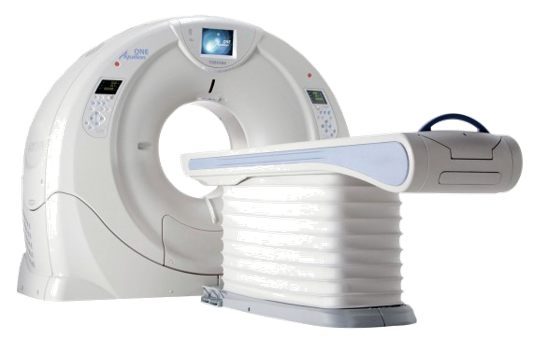
\includegraphics[width=0.45\textwidth]{figures/ct_machine_a.png}}
  \hfill
  \subfloat[]{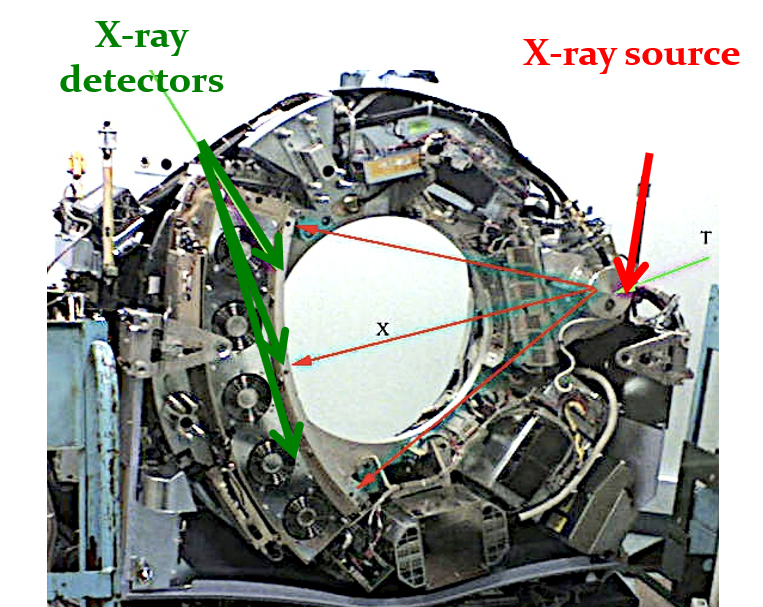
\includegraphics[width=0.45\textwidth]{figures/ct_machine_b.png}}
  \caption{\small{Computed Tomography (CT) scanner (a) and CT scanner with front cover removed (b), exposing the X-ray source and detector array on a rotating gantry.}}
    \label{fig:figures/CT_machine}
\end{figure*}

% harmful radiation
The main disadvantage of CT imaging is that it exposes the patient to a substantial amount of ionizing radiation from X-rays. The radiation dose of a CT scan is the total energy of the X-rays cast onto the patient with sufficient energy to penetrate the structures of the body. The absorbed dose is the energy imparted by ionizing radiation per unit mass of irradiated material. The dose equivalent radiation is a surrogate measure that estimates the hazard to body tissues caused by radiation \cite{mettler2000ct, goo2017dual}. It is cumulative and is quantified in Sievert (Sv) and rem units.
It is now believed that ionizing radiation above a certain threshold may be harmful to the patient \cite{hall2008cancer, davies2011risks, kalra2004strategies}. Studies show that radiation is related to carcinogenesis, which occurs at low doses (\textless 100 mSv) in diagnostic imaging and accounts for an estimated 0.5--0.9\% of cancers. CT-based exams contribute disproportionately to the collective radiation dose of the population. Today, 11\% of diagnostic radiological procedures in the USA are CT examinations. However, their contribution to the collective dose from diagnostic radiology is estimated at 67\% \cite{mettler2000ct}.

The reduction of radiation dose of individual CT scans has become a central clinical and technical issue. In CT imaging, the basic trade-off is between radiation dose and image quality. Lower doses, achieved by fewer X-rays with lower energies, produce imaging artifacts and increased noise, thereby reducing the image quality and limiting its clinical usefulness. Consequently, the clinical indication for CT scan dose determination is the FDA-approved ALARA \textbf{--} As Low As Reasonably Achievable \cite{newman2011alara}. In parallel, many scanning protocols, image reconstruction methods, and clinical evaluation studies have been developed and performed for dose reduction of individual CT scans \cite{shtok2013learned, moore2009adaptive}.

\begin{figure*}[t]
    \centering
    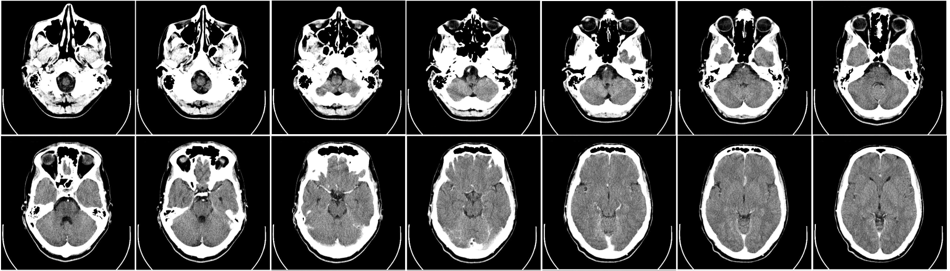
\includegraphics[width=\textwidth]{figures/Brain_CT.png}
    \caption{\small{Axial slices from a CT scan of the brain.}}
    \label{fig:figures/Brain_CT.png}
\end{figure*}

Repeat CT scanning, in which a patient is scanned some time after a baseline scan was acquired, is very common in many clinical situations, including: 1) multi-phase scanning, in which repeated scanning is performed before and after contrast agent injection \cite{kondo2007mdct}; 2) follow-up scanning, in which repeated scanning is performed for disease progression evaluation, e.g., oncology \cite{zhao2009evaluating}; 3) intra-procedural scanning, in which repeated scanning is performed during an intervention to determine anatomical changes and update the location of tools and catheters; 4) post-procedural scanning, in which repeated scanning is performed to evaluate the procedure results vis-à-vis a pre/intra-procedural scan \cite{thomas2010scheduled, hansen2006repeat}; 5) registration scanning, in which repeated scanning is performed at the start and/or at the end of an intervention to align the pre-procedural scan with the patient; 6) ECG-gated heart scanning, in which repeated scanning is performed to compensate for heart motion \cite{desjardins2004ecg, dafni2013methods}. All repeat scan procedures incur in accumulated radiation, which exacerbates the need for radiation reduction.

This thesis aims to take advantage of the significant, untapped opportunities for dose reduction in repeat CT scanning by incorporating data from the baseline scan in the acquisition and analysis of the repeat scan. The potential is shown, for example, in multi-phase and follow-up studies, where reports indicate that many patients that undergo abdominal and pelvic CT scanning have more that one scan on the same day; that 30\% of them have at least three scans in the course of their treatment \cite{davies2011risks}; and that many receive substantial excess radiation dose with no clinical benefit \cite{mettler2000ct}. Dose reduction is of particular importance in pediatric radiology \cite{donnelly2005reducing, chodick2007excess}.

% fractional scanning
The approach by which dose reduction is to be achieved is termed \textit{fractional scanning} in this thesis. 
It is based on sparse sampling of the projections in the view-angle domain, i.e. acquiring only a small fraction of the view angles typically acquired in a regular scan.
This enables reducing the absorbed radiation dose by modulating the X-ray source during gantry rotation, either via current/voltage modulation or fast mechanical collimation.
Fractional scanning is realized in existing CT scanners by tube potential switching and tube current modulation \cite{kalra2004techniques}, and active collimation has been used in radiotherapy \cite{mackie2006history}.
Such alterations to CT scanning firmware and/or hardware are necessary in order to realize the potential of dose reduction using methods presented in this thesis; however, the topic of CT scanner design and control is beyond the scope of this work, which focuses on the algorithmic aspects of leveraging sparse repeat scan data to achieve dose-reduced clinical applications.

\section{The Radon transform}

The integral transform which came to be known as the Radon transform was first described by Johan Radon in 1917 \cite{radon1917determination} and found no practical use until the introduction of the first CT system by Sir Godfrey Newbold Hounsfield and Allan McLeod Cormack in 1971 \cite{maier2018medical}. It is formulated as line integrals parameterized using polar coordinates over the domain of a two-dimensional integrable function $f: \rm I\!R ^2 \rightarrow \rm I\!R $ (see Fig. \ref{fig:figures/radon_a}):
\begin{equation}
\mathcal{R} f(r, \alpha) 
= \int \displaylimits_{(x,y) \in l} f(x,y)\, dl \\
= \int \displaylimits_{(x,y) \in \rm I\!R ^2} { f(x,y)\, \delta(x \cos \alpha + y \sin \alpha - r)}\, dx\, dy
\end{equation}
The resulting two-dimensional function $\mathcal{R} f(r, \alpha)$ is known as the sinogram of $f$, as depicted in Fig. \ref{fig:fractional_a}. Each column of the sinogram is the one-dimensional signal obtained by summation along parallel lines in a specific direction.

The Radon transform is well suited for describing the image formation process underlying CT imaging, which is modeled as an exponential decrease in X-ray intensity as a ray progresses through the object, known as the Beer-Lambert law:
\begin{equation}
I(x) = I_0 \, \exp \left( -\mu \, x \right)
\label{eq:beerlamb}
\end{equation}
where $I_0$ is the initial intensity, $\mu$ is the attenuation coefficient and $I(x)$ represents the intensity after the ray is attenuated through distance $x$. Allowing for non-constant, integrable attenuation $\mu(x,y)$, Eq. \ref{eq:beerlamb} for a ray $l$ spanning between the X-ray source and a detector element becomes
\begin{equation}
I_l = I_0 \, \exp \left( - \int \displaylimits_{(x,y) \in l} \mu(x,y)\, dl \right)
\label{beerlamb}
\end{equation}
 or simply $\mathcal{R} \mu (l) = \log \frac{I_0}{I_l} $. Therefore, post-processing the raw data acquired by a CT scanner, using the photon count at the detector and the known photon count emitted by the source, gives the Radon transform of an axial slice taken from the attenuation function the scanned object. Modern CT scanners are able to acquire many sinogram slices simultaneously. 
 The concept of fractional scanning previously mentioned is realized by sparsely sampling the sinogram slices in the view-angle axis (see Fig. \ref{fig:fractional_b}). 
 %f the repeat scan sinogram data is acquired using this pattern by modulating the X-ray source during its rotation, the reduction of ionizing radiation to which a patient is exposed would be significant - by an order of magnitude or more, depending on the sparsity of sampling and speed of modulation.
 
 The inversion of the Radon transform for image reconstruction can be achieved using different methods, most notably the Filtered Back-Projection algorithm which relies on a theorem relating the Radon and Fourier transforms (Fourier Slice Theorem).
 
\begin{figure*}[t]
  \centering
  \subfloat[]{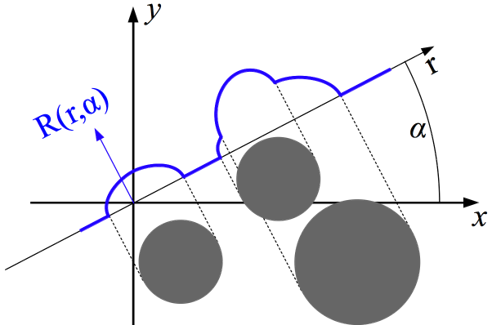
\includegraphics[width=0.45\textwidth]{figures/radon_a.png}
  \label{fig:figures/radon_a}}
  \hfill
  \subfloat[]{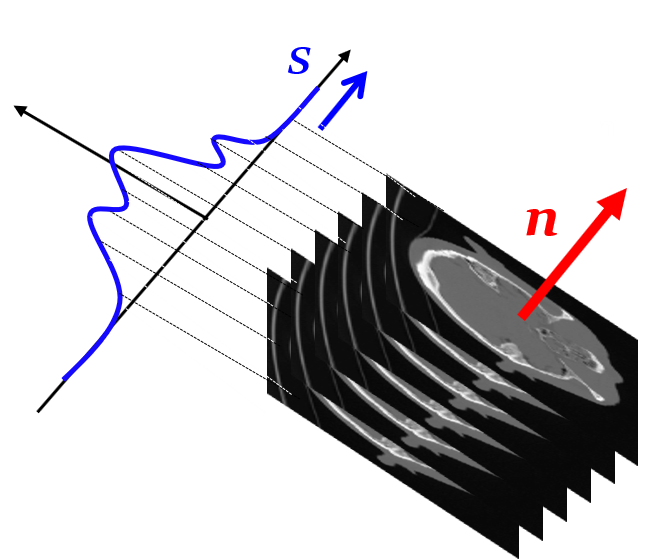
\includegraphics[width=0.45\textwidth]{figures/radon_b.png}
  \label{fig:figures/radon_b}}
  \caption{\small{Illustration of the Radon transform for a single direction: (a) The two-dimensional Radon transform of a planar image is achieved by summation along parallel lines perpendicular to an axis $r$ at an angle $\alpha$ relative to the positive $x$ direction, producing a one-dimensional signal. (b) The three-dimensional Radon transform of a volumetric image involves summation along parallel planes having normal vector $\hat{n}$, producing a one-dimensional signal as well.}}
    \label{fig:figures/radon}
\end{figure*}


 The two-dimensional Radon transform is extended to three dimensions as follows. The Radon transform of an integrable function $f: \rm I\!R ^3 \rightarrow \rm I\!R $ involves integration along parallel planes (see Fig. \ref{fig:figures/radon_b}):
 \begin{equation}
    \mathcal{R}^{3D} f(s, \hat{n}) 
    = \int \displaylimits_{\textbf{r}\, \in H(\hat{n}, s)} f(\textbf{r})\, dA
 \end{equation}
 where $H(\hat{n}, s) = \{ \textbf{r} \in \rm I\!R ^3 : \textbf{r} \cdot \hat{n} = s\}$ and integration is performed within each plane $H(\hat{n}, s)$. For a constant projection direction $\hat{n}$, $\mathcal{R}^{3D} f(s, \hat{n})$ is a one-dimensional signal in $s$, similarly to the two-dimensional Radon transform. As noted by \cite{mooser2013estimation}, the values of $\mathcal{R}^{3D} f(s, \hat{n})$ can be calculated directly from slice sinograms stack of a volume without the need to reconstruct the volume image and carry out planar integration. This is achieved by performing two-dimensional Radon transforms on slices from the $r-z$ plane of the sinograms stack. This relation allows calculating the three-dimensional Radon transform of a fractionally scanned volume without first going through volume reconstruction - which would have been impossible due to the sparsity of the data collected.

\begin{figure*}[t]
  \centering
  \subfloat[]{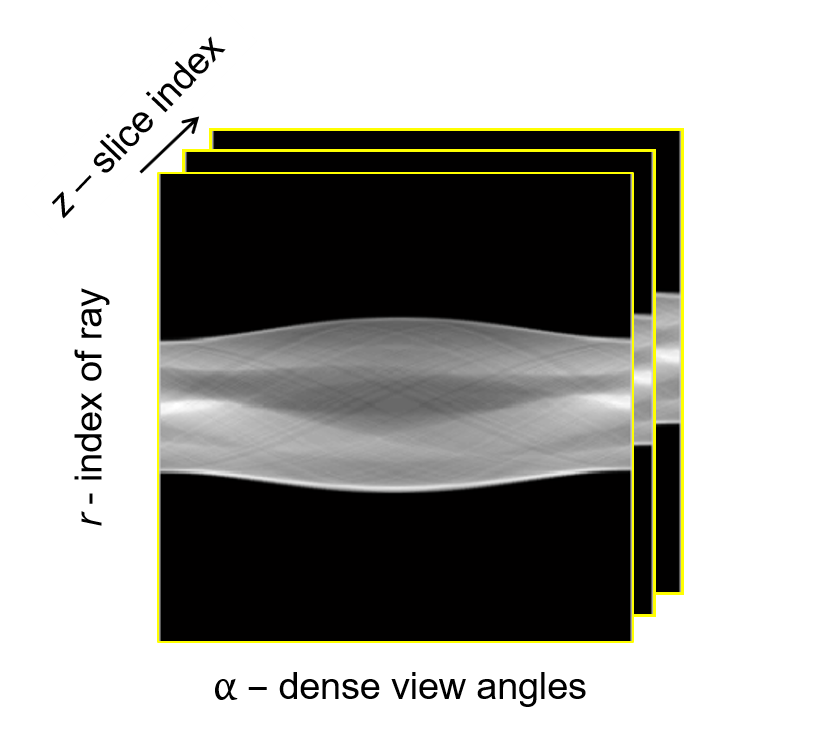
\includegraphics[width=0.45\textwidth]{figures/fractional_a.png}
  \label{fig:fractional_a}}
  \hfill
  \subfloat[]{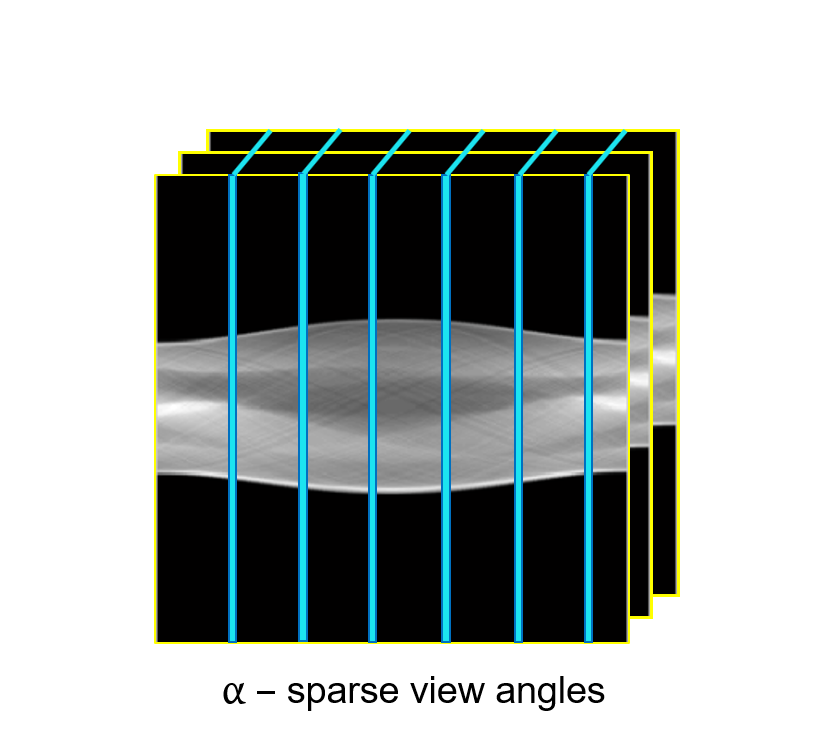
\includegraphics[width=0.45\textwidth]{figures/fractional_b.png}
  \label{fig:fractional_b}}
  \caption{\small{Radon transforms of two dimensional images (sinograms), representing slices of a volume along the z direction. (a) Full sinograms, densely sampled in the view angle direction. (b) Blue lines on the sinograms highlighting the regions acquired during sparse view angle sampling in fractional scanning.}}
    \label{fig:figures/fractional}
\end{figure*}

\section{Previous work}

The literature reviewed in this section TODO

Medical image registration has been studied extensively, with several approaches emerging \cite{maintz1998survey}.
\textbf{Feature-based} methods compute the rigid transformation by matching points defined in volumetric medical images, usually of fiducials or natural features, and minimizing the sum of their pairwise distances. Since these methods require the explicit identification and matching of points, their scope is limited to selected clinical scenarios. 
\textbf{Intensity-based} methods perform the registration by comparing the intensity values of both images, a technique which has become dominant in image registration over the past decades \cite{viergever2016survey}. To yield adequate results, they require both volumetric images to be of good quality, be free of image reconstruction artifacts, and have small scanned subject/pose discrepancies.

Specific to the domain of medical images based on radiography (X-ray and CT imaging), \textbf{intensity-based 2D X-ray to 3D CT} registration methods have been developed. Some are in routine clinical use for image-guided therapy and for patient positioning during treatment (see \cite{markelj2012review} for a comprehensive survey). In all cases, the matching procedure requires at least two (and often more) X-ray images of sufficient quality for the matching. The drawbacks of these methods are that they may use different hardware for CT and X-ray acquisition, and that they require set-up time.

\textbf{Radon-space methods}, also called sinogram or projection-space methods, use the CT scans Radon transform representation (sinograms) for the registration. They are not subject to image reconstruction artifacts and have the potential to yield robust and accurate results with greatly reduced doses.
Freiman et al. \cite{freiman2011spectral} describe a 2D/3D registration method for X-ray to CT scans that uses invariant Fourier space features to find the transformation parameters by out-of-plane coarse registration followed by in-plane fine registration. 
Mao et al. \cite{mao2007ct} describe a slice-by-slice registration method in 2D Radon space and its extension to 3D for small angles.
Mooser et al. \cite{mooser2013estimation} propose an iterative optimization method to compute the registration parameters in 3D Radon space for full scans. 
You et al. \cite{you1998image} investigate the invariant properties of rigid movement in image and Radon space. 
Based on this work, Lu, Fitchard et al. \cite{lu1999image, fitchard1998registration, fitchard1999six} use Fourier phase matching to iteratively compute the rigid registration parameters by decomposing the 3D problem into a series of 2D in-plane registrations. The method is limited to small transformations. 

More recently, Wein et al. \cite{wein2011detecting}, Aichert et al. \cite{aichert2014redundancies,aichert2015epipolar}, and Debbler et al \cite{debbeler2013new} use directed epipolar geometry to establish consistency metrics between different projection views for the detection of mid-scan patient motion. However, inter-scan registration is not addressed. 
The 2D Radon transform was shown to be very useful for pattern matching and registration of 2D images, both in terms of accuracy, convergence range and noise robustness \cite{nacereddine2015similarity, wan2010fast}. However, the authors do not indicate how their methods can be extended to 3D and to real sinogram data. 

Deformable registration methods in projection space are also addressed. 
Osorio et al. \cite{osorio2007non} describe a Fourier space based on full CT scans.
Zhang et al. \cite{zhang2014few} present a method that iteratively matches the repeat scan projection to the re-projected deformed baseline. The method requires a preceding rigid registration step to allow convergence of the deformation field to the optimal solution.  
Large reductions in radiation dose have been shown for 3D/2D registration between CT and C-arm fluoroscopy \cite{uneri2014evaluation}.

Clinical applications enabled by the ability to register a sparse repeat scan to a baseline CT scan are present in this thesis, namely -- rigid and flexible needle localization. Localization of surgical instruments in CT imaging, and needles in particular, has been addressed in a variety of ways. The needle is usually localized in image space, and so is often required to be inserted in the axial imaging plane (in-plane insertion), which forces the radiologist to adjust the setup repeatedly and re-scan until a suitable orientation is found \cite{walsh2011smaller}. Steering the needle inside the tissue toward the target can be achieved manually by the radiologist under passive guidance, or by robotic steering in closed loop with the imaging. A commercial CT navigation device, SimpliCT by NeoRad \cite{simpliCT}, implements laser steering to guide the radiologist during manual insertion by aligning the needle with the laser direction. In \cite{schubert2013ct}, an optical tracking system uses surface markers to allow feedback of the needle orientation during the intervention. Another approach is to optically over-lay the CT image on top of the patient using a semi-transparent mirror, thereby providing the physician with visual guidance during manual needle insertion \cite{fichtinger2005image}.

Several works describe specific methods to localize the needle shape in reconstructed CT images, relying on acquisition of full repeat scan and reconstruction of the image for each localization of the needle.
Hou et al. \cite{huo2015shape} reconstruct the bevel-tip flexible needle trajectory from full CT slices by localizing points at which the needle intersects slice planes, and fitting a four-order polynomial to the collection of 3D points.
Yaniv et al. \cite{yaniv2010needle} describe a system in which embedded electromagnetic fiducials are used for needle tracking under CT guidance, with operator input required to identify the needle tip in a full CT scan taken in-situ.

The needle shape can be used for control loop feedback in image guided actuated intervention systems.
Ben-David et al. \cite{ben2018evaluation} describe a robotic system for flexible needle insertion under CT guidance. A dual guiding mechanism is composed of a driver which advances the needle while a positioning unit steers it during insertion. A pre-planned 3D trajectory is executed and amended during the insertion based on full repeated CT scans. Earlier work by Glozman et al. \cite{glozman2007image} describes robotic flexible needle steering and a needle-tissue mechanical interaction model, where feedback is based on 2D in-plane imaging of the needle.

\section{Research goals}

\textbf{The first goal of this thesis is to develop and validate an algorithm for rigid registration in repeat CT scanning procedures based on Radon-space methods achieving an X-ray dose reduction.}

The focus of this thesis is to develop methods taking advantage of the information in the baseline scans to reduce the radiation dose required in the follow-up scan. Rigid registration is a cornerstone of computational radiology, and in the case of repeat CT scanning, is an essential preliminary stage in incorporating the information from the baseline and repeat scans in order to produce any clinical value.

\textbf{The second goal is to develop intra-operative needle tracking methods to allow patient tracking and needle localization.}

The needle tracking solution for interventional radiology realizes the potential of Radon-space rigid registration for dose reduction in a clinical context.

\section{Thesis overview and novelty}

This thesis presents a novel rigid registration method for repeat CT scanning, and a novel application enabled by it in CT guided interventions.

\textbf{The Radon-space rigid registration method} computes the 6 degrees-of-freedom rigid registration between a baseline scan and a repeat scan without repeat scan image reconstruction and using fractional scanning, which reduces the X-ray dose to which the patient is exposed during the repeat scan.
It is presented in two parts: the first is a method overview for parallel rays geometry with preliminary results using simulated sinogram data obtained from reconstructed CT images. The second part is a theoretical extension to fan- and cone-beam geometries, along with an extensive validation study on parallel rays sinogram data obtained in collaboration with a CT manufacturer - GE Healthcare Haifa.
 
The main advantages of this method are that it: 
1) out-performs image space registration under sparse sampling conditions;
2) supports much larger transformations than image space registration; 
3) allows for a theoretical dose reduction beyond $\times$100 by combining low tube current scanning and fractional scanning.

\textbf{The rigid needle localization method} builds upon the rigid registration method.
It relies on a spherical marker attached to the needle at a known distance from the tip. The marker is detected in projection difference images, which are generated using the rigid registration obtained using the previous method, and localized in 3D space. Then, the rigid needle direction in 3D space is computed as an intersection of planes associated with the needle projections in the projection difference images.

The main advantages of this method are: 1) it enables existing clinical procedures in interventional radiology to benefit from the potential of X-ray dose reduction; and 2) it accurately localizes the needle with respect to an artifact free baseline scan, without reconstructing the repeat scan image prone to metallic artifacts due to the needle.

\textbf{The flexible needle localization method} extends the rigid needle localization method to expand the range of applicable procedures to those requiring a flexible needle, such as obtaining biopsies of deeply situated targets where sensitive tissue structures must be avoided.
It divides the needle trajectory into short segments and incrementally traces control points along it to generate a curve in 3D space following the needle path.

The main advantage of this method is expanding the applicable procedures of needle based CT-guided interventions to those requiring flexible needles.


\section{Thesis organization}

The rest of this thesis consists of four articles describing the methods listed in the previous section, a discussion, and a list of references. It is organized as follows: 

\textbf{Chapter \ref{chapters/c127-2014-miccai-radon-registration.pdf}}: Reduced-dose patient to baseline CT rigid registration in 3D Radon space.
G. Medan, A. Kronman, L. Joskowicz. \textit{International Conference on Medical Image Computing and Computer-Assisted Intervention, p 291-298, 2014.}

\textbf{Chapter \ref{chapters/Sparse_3D_Radon_Space_Rigid_Registration.pdf}}: Sparse 3D Radon space rigid registration of CT scans: Method and Validation Study.
G. Medan, N. Shamul, L. Joskowicz. \textit{IEEE Trans. Med. Imaging 36, no. 2 (2017): 497-506.}

\textbf{Chapter \ref{chapters/Reduced-dose_imageless_needle.pdf}}: Reduced-Dose imageless needle and patient tracking in interventional CT procedures.
G. Medan, L. Joskowicz. \textit{IEEE Trans. Med. Imaging 36, no. 12 (2017): 2449-2456.}

\textbf{Chapter \ref{chapters/Flexible_needle.pdf}}: Flexible needle and patient tracking using fractional scanning for reduced dose in interventional CT procedures. \textit{Guy Medan and Leo Joskowicz.}

\textbf{Chapter \ref{ch:conclusions}}: Conclusions

\textbf{References}

\pagestyle{plain}
\cleardoublepage

\addpdfchapter[Reduced-dose patient to baseline CT rigid registration in 3D Radon space]%
{\textbf{Published as}: G. Medan, A. Kronman, L. Joskowicz. “Reduced-dose patient to baseline CT rigid registration in 3D Radon space”. \textit{Proc. 17th Int. Conf. Medical Image Computing and Computer-Assisted Intervention}, pp 291-298, 2014. }%
{chapters/c127-2014-miccai-radon-registration.pdf}
{-}

\addpdfchapter[Sparse 3D Radon Space Rigid Registration of CT Scans: Method and Validation Study]%
{\textbf{Published as}: G. Medan, N. Shamul, L. Joskowicz. "Reduced-dose patient to baseline CT rigid registration in 3D Radon space". \textit{IEEE Trans. Med. Imaging} 36, no. 2, pp 497-506, 2017.}%
{chapters/Sparse_3D_Radon_Space_Rigid_Registration.pdf}
{-}

\addpdfchapter[Reduced-Dose Imageless Needle and Patient Tracking in Interventional CT Procedures]%
{\textbf{Published as}: G. Medan, L. Joskowicz. "Reduced-Dose Imageless Needle and Patient Tracking in Interventional CT Procedures". \textit{IEEE Trans. Med. Imaging} 36, no. 12, pp 2449-2456, 2017.}%
{chapters/Reduced-dose_imageless_needle.pdf}
{-}

\addpdfchapter[Flexible needle and patient tracking using fractional scanning in interventional CT procedures]
{By Guy Medan and Leo Joskowicz (\textit{unpublished}).}
{chapters/Flexible_needle_ipcai2019_for_thesis.pdf}
{-}


\cleardoublepage
\chapter{Conclusions}

\label{ch:conclusions}

\section{Summary}

The pervasiveness of CT studies in routine clinical use has focused much attention on methods to mitigate its most prominent drawback - the increased risk of cancer due to exposure to ionizing radiation. 
Repeat CT scanning, while very common throughout the clinical work flow of diagnosis, treatment and follow-up, offers a relatively untapped opportunity for dose reduction by incorporating information from previous scans of the patient during acquisition of a repeat scan.
This thesis presents methods for repeat CT scanning which rely on a novel approach to X-ray dose reduction: fractional scanning in the view-angle domain. With this approach the dose absorbed by the patient in the repeat scan could be reduced by at least an order of magnitude, by acquiring only a fraction of the projection data necessary for image reconstruction and using algorithms designed specifically for this domain.

\textbf{The Radon-space rigid registration method} is the basis for any comparison between the baseline scan and fractional repeat scans.
Our study on real sinogram data from phantom scans shows that it out-performs image space registration under sparse sampling conditions, and is able to recover larger transformations than image space registration.

\textbf{The rigid needle localization method} builds upon the Radon space registration method and relies on a spherical marker attached to the needle at a known distance from the tip as a starting point for the localization. This is achieved using projection difference images, computed by comparing the baseline and repeat scans based on the rigid registration calculated by the first method. The needle trajectory is then traced in 3D space from the projection difference images. The trajectory can then be displayed as an augmentation of the baseline scan (see Fig \ref{fig:figures/needle+patient_tracking.png}). Our experimental results on five scans of an abdomen phantom show it is able to localize the needle tip with error of up to 2mm for out-of-plane insertions without reconstructing the repeat scan image.

\textbf{The flexible needle localization method} extends the rigid needle localization method to flexible needles by establishing control points along the needle path to calculate a bezier curve representing the trajectory. Experiments on seven scans of an abdomen phantom and with two types of flexible needles show an average tip localization error of 2.4 mm.

\begin{figure*}
    \centering
    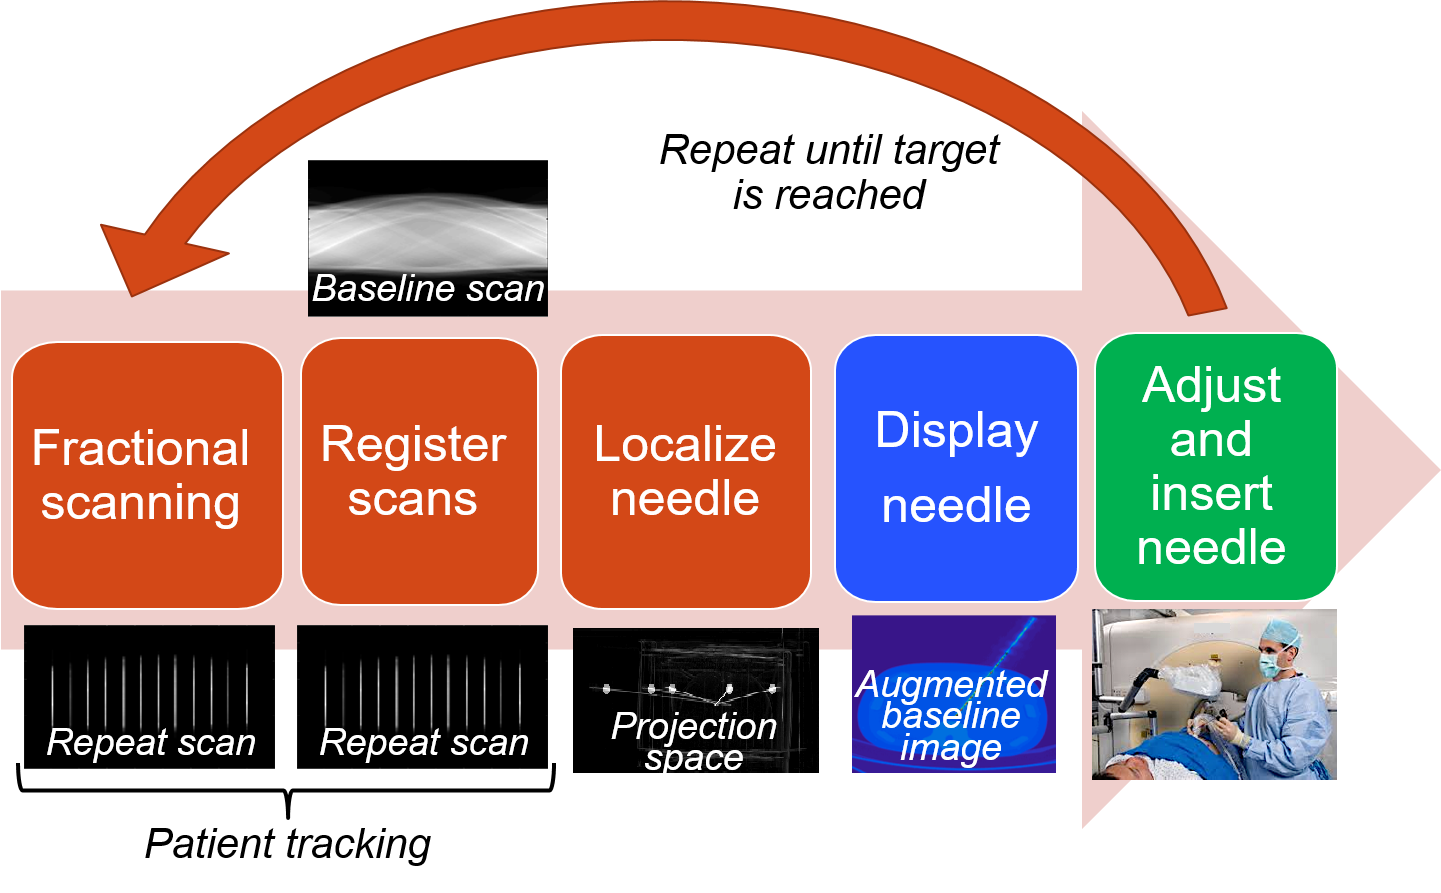
\includegraphics[width=15cm]{figures/needle+patient_tracking.png}
    \caption{\small{Illustration of image-less needle and patient tracking process in interventional radiology.}
}
    \label{fig:figures/needle+patient_tracking.png}
\end{figure*}

\section{Future work}

The methods described in this thesis take advantage of sparse sampling in the view-angle domain during the CT acquisition process. However, to achieve the potential of substantial dose reduction, the scanning protocol and hardware itself must be altered in ways that are beyond the scope of this thesis. For example, some variants of dual-energy CT scanners switch the tube voltage between higher voltage (140kV) to lower voltage (80kV) every 1$^\circ$ 
\cite{goo2017dual}. By alternatively switching the voltage between high and low and with a wider angular spacing of 10$^\circ$-20$^\circ$, an X-ray dose reduction of $\times$10-50 can be achieved.

A different application to the low-dose rigid registration algorithm presented in this thesis is investigated by Shamul et al. \cite{shamul2017radon}. The goal of this work is to combine the baseline scan data with fractional repeat scanning to reconstruct CT images of the patient such that they incorporate any changes in the anatomy that may have occurred since the baseline scan, while achieving an X-ray dose reduction compared to a full repeat scan. In this approach a map of changed regions is computed based on comparisons in Radon space (made possible thanks to Radon space rigid registration), and consequently sparse scanning is performed such that only rays passing through the changed regions are acquired, enabling the reduction of X-ray dose. Then, the repeat and baseline data is combined in Radon space so that an image reconstruction can be computed using well known reconstruction methods. It is noted that this approach extends the hardware requirements from a CT scanner to not only support fractional scanning of view angles, but also to dynamically adjust its collimator as the gantry rotates so that only beams of interest are scanned.

Further work yet to be published by Adelman et al. extends rigid registration in Radon space to simultaneous deformable registration and image reconstruction based on a similar scheme of sparse view angles scanning and algebraic image reconstruction. This work has the potential to bring the promise of dose reduced applications to clinical procedures in which deformations cannot be neglected.

We expect that our approach to X-ray dose reduction will have a significant impact on the ongoing effort to lower doses of ionizing radiation in radiology, as manufacturers adopt new technologies in CT scanners enabling the rise of novel algorithms promising the benefit of reduced radiation-related risk to patients.

%\appendix
% appendices come here


\addcontentsline{toc}{chapter}{Bibliography}
\bibliographystyle{ieeetr_last_name_first}
\bibliography{thesis.bib}

\cleardoublepage

\includepdf[pages=last-1]{chapters/hebrew_intro.pdf} % reverse order

\end{document}